\documentclass[a4paper]{article}

\usepackage{fullpage} % Package to use full page
\usepackage{parskip} % Package to tweak paragraph skipping
\usepackage{tikz} % Package for drawing
\usepackage{amsmath}
\usepackage{hyperref}

\title{SAP Challenge}
\author{Kou Wen}

\begin{document}

\maketitle

\section{Introduction}

The fancy title of SAP Challenge is \emph{Which Novel Do I Belong To?}. Translating the title into machine learning language is classifying the documents into correct categories (text classification). There are quite a mount of classification algorithms which can be applied to solve this issue, e.g. KNN, Logistic regression (For multiple classes, it is preferred as SoftMax), decision tree, linear discriminant analysis, SVM, etc. Those approaches can be regarded as linear approach which assumes the data is linear separable. But if kernel trick is preferred, that is another kind of story. The assumption is that those data is not linear separable that no appropriate hyperplane can be learnt using the above approaches, so kernel trick would seek for another feature space which can linearize the feature from the original feature space to make the problem linear separable again. But in this task, I would like to adopt nowadays fashion approach Convolutional Neural Network aka. \emph{CNN}. In this task, I would like to tackle the different layers: convolutional layers, rectifier linear unit(ReLU) layers, pooling layers, fully connected layers, etc and manipulate the learnable parameters for example to try how many filters is suitable for each convolutional layers to seek a good CNN structure which can well solve classification problem.

In the \emph{Which Novel Do I Belong To?}, there is another critical issue in feature extraction. The representation of each text is not natural English word since they have been encrypted so it is not possible to apply any pretrained word embedding as feature directly as other typical text classification problem. But it is said "each character has a deterministic mapping" which means each word e.g. "boy" could always be mapped as "sua", so character level feature extraction can be suitable for this task. X. Zhang \cite{ZhangZL15} applied one-hot to encode each char in a char table as basic feature.

In section\ref{algoDetail}, the detail of the algorithms is described. In section\ref{exp}, experiments and analysis are explained. In section\ref{conclusion}, conclusion is summarized.

\section{Algorithm Detail}\label{algoDetail}

\subsection{Feature Extraction}
In this task, I applied one-hot feature extraction method to encode char in char dictionary:
\begin{equation}
D = \{'a': \mathbf{a},'b': \mathbf{b},'c': \mathbf{c},'d': \mathbf{d}....\}
\end{equation}
For this task, the char dictionary will contain only 26 alphabet characters, so the feature vector is $R^{26 \times 1}$. Each feature matrix of each article will be $R^{26 \times n}$ where $n$ is the article length.

This feature extraction would make since each word including spaces or other will deterministically be mapped to another aphetic space 

\subsection{CNN architecture}

The definition of the limit of $f(x)$ at $x=a$ denoted as $f'(a)$ is:

\begin{equation}
f'(a) = \lim_{h\to0}\frac{f(a+h)-f(a)}{h}
\end{equation}

The following code can be used in sage to give the above limit:

\begin{verbatim}
def illustrate(f, a):
    """
    Function to take a function and illustrate the limiting definition of a derivative at a given point.
    """
    lst = []
    for h in srange(.01, 3, .01):
    	lst.append([h,(f(a+h)-f(a))/h])
    return list_plot(lst, axes_labels=['$x$','$\\frac{f(%.02f+h)-f(%.02f)}{h}$' % (a,a)])
\end{verbatim}

\begin{figure}[!htbp]
\begin{center}
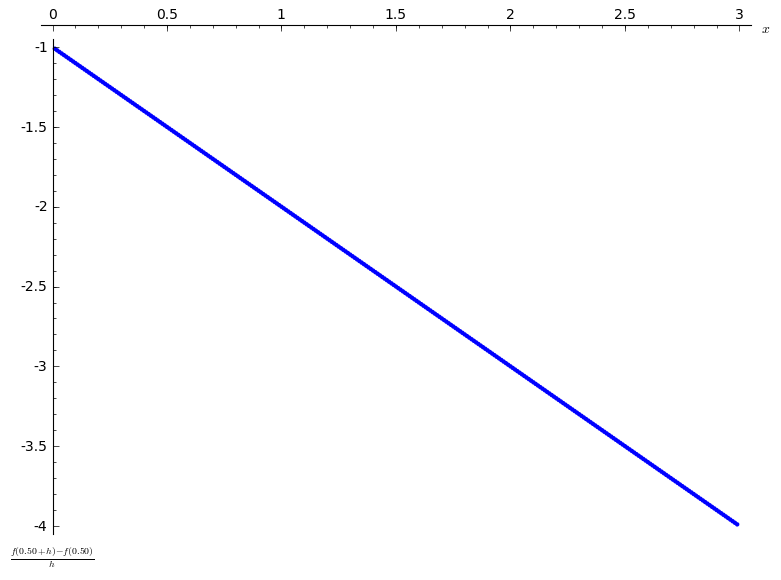
\includegraphics[width=8cm]{sage1.png}
\end{center}
\caption{The derivative of $f(x)=1-x^2$ at $x=.5$ converging to -1 as $h\to0$.}
\end{figure}

If we want to plot the tangent at a point $\alpha$ to a function we can use the following:

\begin{align}
y=&ax+b&&\text{(definition of a straight line)}\nonumber\\
  &f'(a)x+b&&\text{(definition of the derivative)}\nonumber\\
  &f'(a)x+f(a)-f'(a)a&&\text{(we know that the line intersects $f$ at $(a,f(a))$}\nonumber
\end{align}

We can combine this with the approach of the previous piece of code to see how the tangential line converges as the limiting definition of the derivative converges:

\begin{verbatim}
def convergetangentialline(f, a, x1, x2, nbrofplots=50, epsilon=.1):
    """
    Function to make a tangential line converge
    """
    clrs = rainbow(nbrofplots)
    k = 0
    h = epsilon
    p = plot(f, x, x1, x2)
    while k < nbrofplots:
        tangent(x) = fdash(f, a, h) * x + f(a) - fdash(f, a, h) * a
        p += plot(tangent(x), x, x1, x2, color=clrs[k])
        h += epsilon
        k += 1
    return p
\end{verbatim}

The plot shown in Figure \ref{lines} shows how the lines shown converge to the actual tangent to $1-x^2$ as $x=2$ (the red line is the `closest' curve).

\begin{figure}[!htbp]
\begin{center}
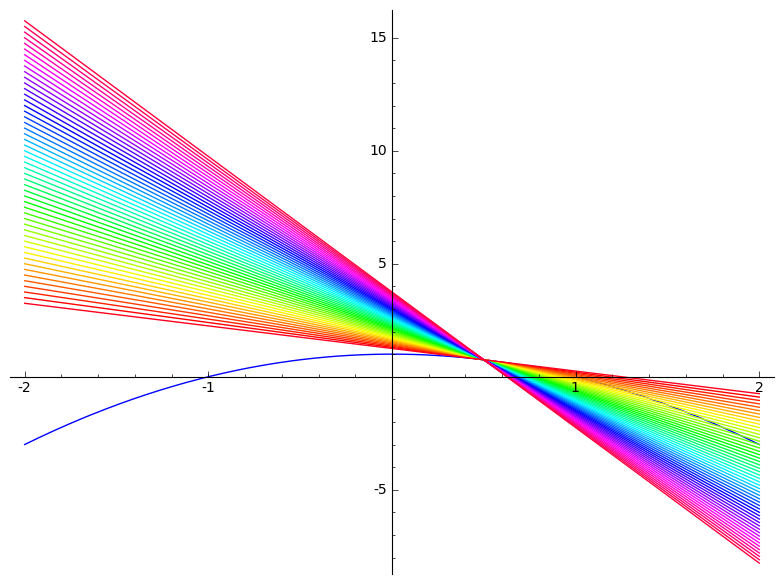
\includegraphics[width=8cm]{sage0.png}
\end{center}
\caption{Lines converging to the tangent curve as $h\to0$.}\label{lines}
\end{figure}

Note here that the last plot is given using the \textbf{real} definition of the derivative and not the approximation.

\section{Experiment}\label{exp}

In this report I have explored the limiting definition of the limit showing how as $h\to 0$ we can visualise the derivative of a function. The code involved \url{https://sage.maths.cf.ac.uk/home/pub/18/} uses the differentiation capabilities of Sage but also the plotting abilities.

There are various other aspects that could be explored such as symbolic differentiation rules. For example:

$$\frac{dx^n}{dx}=(n+1)x^{n}\text{ if }x\ne-1$$

Furthermore it is interesting to not that there exists some functions that \textbf{are not} differentiable at a point such as the function $f(x)=\sin(1/x)$ which is not differentiable at $x=0$. A plot of this function is shown in Figure \ref{notdiff}.

\begin{figure}[!htbp]
\begin{center}
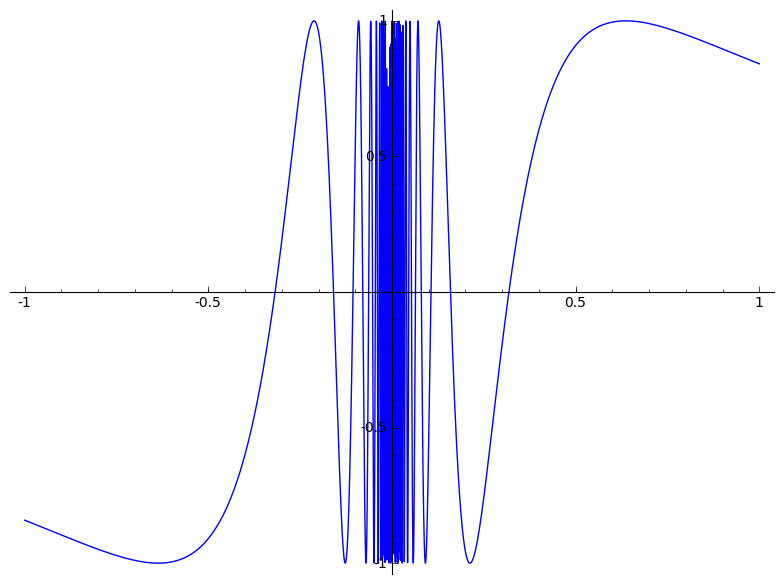
\includegraphics[width=8cm]{sage2.png}
\end{center}
\caption{None differentiable function at $x=0$.}\label{notdiff}
\end{figure}

\section{Conclusion}\label{conclusion}


\bibliographystyle{plain}
\bibliography{bibliography.bib}
\end{document}
